\begin{frame}
	\frametitle{Procedimento 01}
	\framesubtitle{Desempenho}
	\only<1>{
		\begin{itemize}
			\item Em se tratando das escalas, se verificou que BARK apresentou melhor desempenho em todas as combinações testadas.
			\item A combinação \textbf{\textit{wavelet} + Bark} apresentou, consistentemente, \textbf{melhor} viabilidade do que as respectivas combinações \textbf{\textit{wavelet + Mel}}.
			\item De todas as possibilidades verificadas a \textbf{\textit{wavelet} haar + Bark} apresentou o melhor desempenho.
		\end{itemize}
		
		\begin{table}
			\definecolor{tcB}{rgb}{0.447059,0.74902,0.266667}
			\definecolor{tcA}{rgb}{0.65098,0.65098,0.65098}
			\definecolor{tcC}{rgb}{1,0.94902,0}
			\centering
			\begin{tabular}{|c|c|c|c|}\hline
				% use packages: color,colortbl
				\rowcolor{tcA}
				Wavelet & G1 & G2 & Distância do ponto (1,0)\\\hline
				\rowcolor{tcB}
				haar & 0.93615 & 4.68316e-310 & 0.0638503\\\hline
				\multicolumn{1}{|>{\columncolor{tcC}}c|}{daub4} & \multicolumn{1}{>{\columncolor{tcC}}c|}{0.928088} & \multicolumn{1}{>{\columncolor{tcC}}c|}{4.68316e-310} & \multicolumn{1}{>{\columncolor{tcC}}c|}{0.0719123}\\\hline
				\multicolumn{1}{|>{\columncolor{tcC}}c|}{daub6} & \multicolumn{1}{>{\columncolor{tcC}}c|}{0.927885} & \multicolumn{1}{>{\columncolor{tcC}}c|}{4.68316e-310} & \multicolumn{1}{>{\columncolor{tcC}}c|}{0.072115}\\\hline
				\multicolumn{1}{|>{\columncolor{tcC}}c|}{coif6} & \multicolumn{1}{>{\columncolor{tcC}}c|}{0.927823} & \multicolumn{1}{>{\columncolor{tcC}}c|}{4.68316e-310} & \multicolumn{1}{>{\columncolor{tcC}}c|}{0.072177}\\\hline
				\multicolumn{1}{|>{\columncolor{tcC}}c|}{sym8} & \multicolumn{1}{>{\columncolor{tcC}}c|}{0.92769} & \multicolumn{1}{>{\columncolor{tcC}}c|}{4.68316e-310} & \multicolumn{1}{>{\columncolor{tcC}}c|}{0.0723096}\\\hline
				\multicolumn{1}{|>{\columncolor{tcC}}c|}{\tiny\vdots} & \multicolumn{1}{>{\columncolor{tcC}}c|}{\tiny\vdots} & \multicolumn{1}{>{\columncolor{tcC}}c|}{\tiny\vdots} & \multicolumn{1}{>{\columncolor{tcC}}c|}{\tiny\vdots}\\\hline
			\end{tabular}
		\end{table}
	}
	\only<2>{
		\begin{figure}
			\centering
			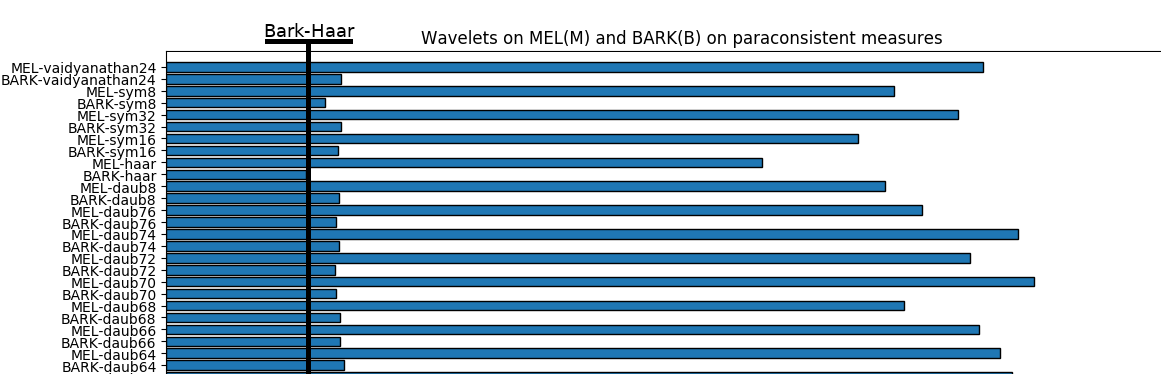
\includegraphics[width=0.7\linewidth]{images/results/paraconsistentPlane/ParaconsistentPart00}
			\caption{Quanto menor o comprimento horizontal das barras na cor azul, melhor a separabilidade entre as classes.}
		\end{figure}
	}
	
	\only<3>{
		\begin{figure}
			\centering
			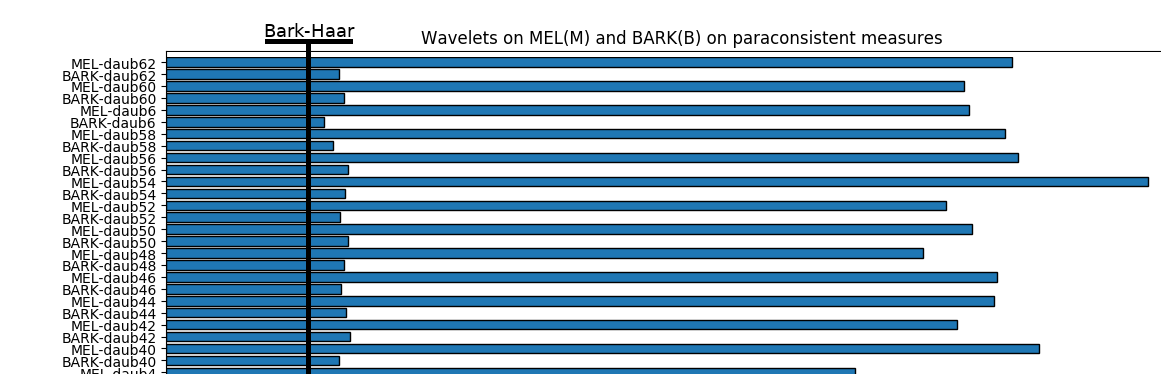
\includegraphics[width=0.7\linewidth]{images/results/paraconsistentPlane/ParaconsistentPart01}
			\caption{Quanto menor o comprimento horizontal das barras na cor azul, melhor a separabilidade entre as classes.}
		\end{figure}
	}
	
	\only<4>{
		\begin{figure}
			\centering
			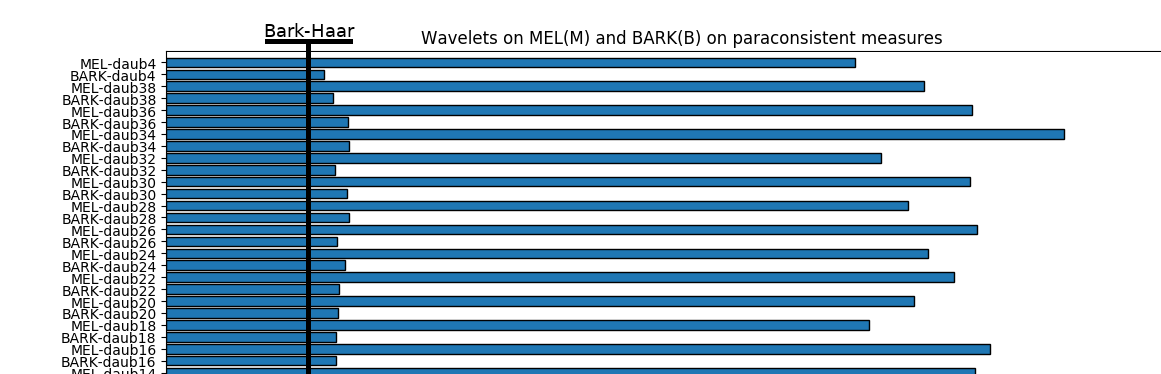
\includegraphics[width=0.7\linewidth]{images/results/paraconsistentPlane/ParaconsistentPart02}
			\caption{Quanto menor o comprimento horizontal das barras na cor azul, melhor a separabilidade entre as classes.}
		\end{figure}
	}
	
	\only<5>{
		\begin{figure}
			\centering
			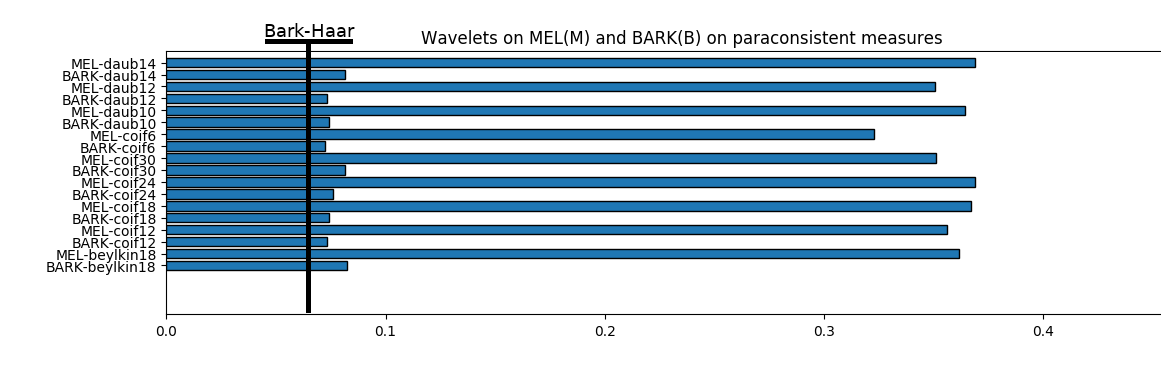
\includegraphics[width=0.7\linewidth]{images/results/paraconsistentPlane/ParaconsistentPart03}
			\caption{Quanto menor o comprimento horizontal das barras na cor azul, melhor a separabilidade entre as classes.}
		\end{figure}
	}
	
	\only<6>{
		\framesubtitle{Síntese}
		\begin{columns}
			\column{0.5\textwidth}
			\begin{itemize}
				\item \textbf{Haar} e \textbf{Daubechies 42} proporcionaram, respectivamente, os melhores e os piores resultados associados com a escala Bark.
				\item Com a escala \textit{Mel}, \textbf{Haar} foi o melhor filtro e \textbf{Daubechies 54} o pior.
			\end{itemize}
			
			\par \textbf{\textit{Wavelet} Haar}
			\begin{itemize}
				\item Filtro de ordem 1
				\item Resposta perfeitamente linear.
				\item Contaminação por bandas adjacentes.
				\item Curva de resposta em frequência mais distante da ideal.
			\end{itemize}
			
			\column{0.5\textwidth}
			\par Portanto, experimentalmente, constatou-se que uma resposta em frequência não-rigorosa associada à uma resposta em fase perfeitamente linear é a melhor alternativa.\newline
			
			\par A \textbf{característica ruidosa} dos sinais regravados, contendo, ao contrário das vozes originais, notórios componentes de altas frequências, é melhor detectada com uma escala mais apropriada ao tratamento de áudio em geral e não voz somente.	
		\end{columns}
	}
	
\end{frame}